
% 主要写:研究区域与数据处理
\section{研究区域}
\subsection{研究区域介绍}
\begin{figure}[H]
    \centering
    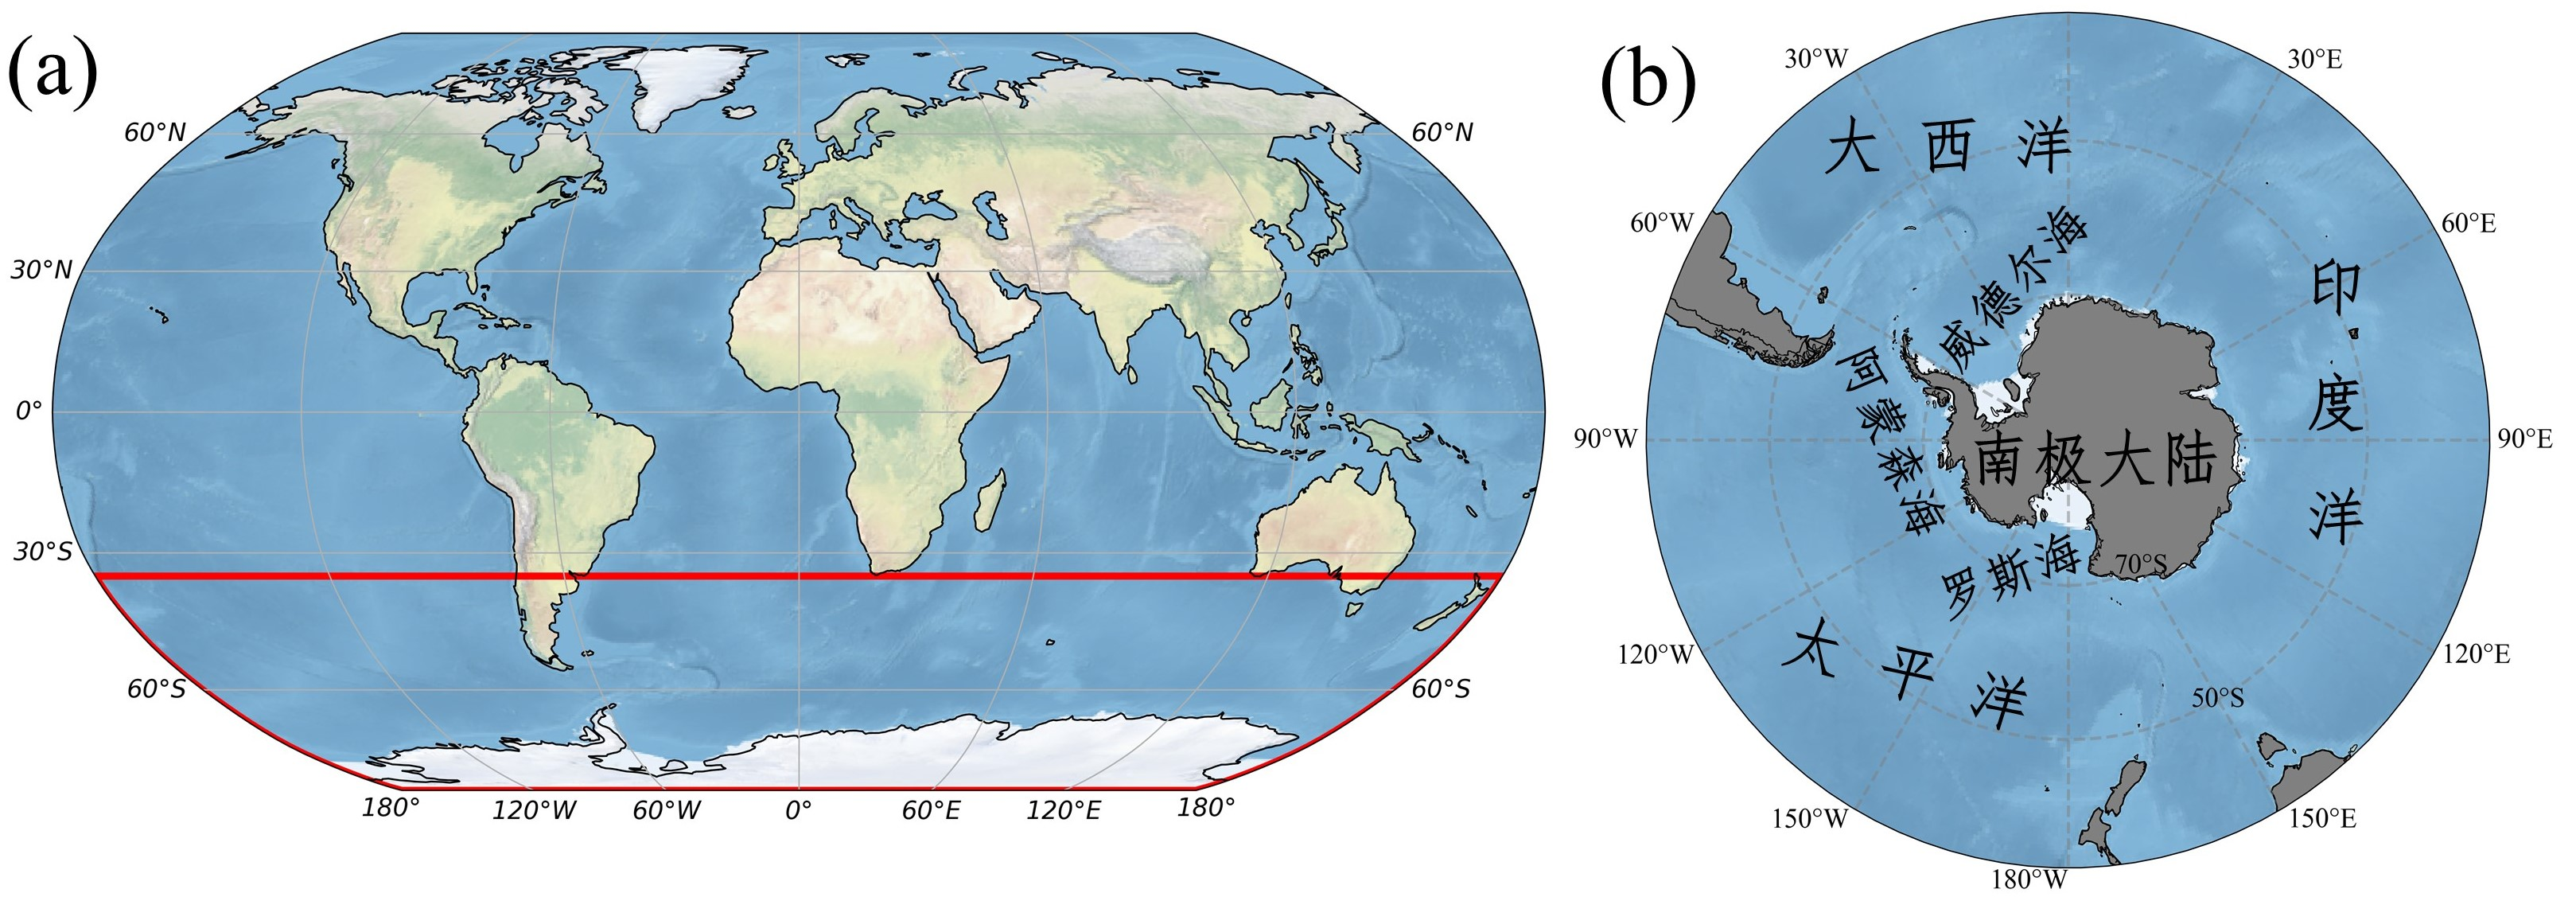
\includegraphics[width=\linewidth]{figure/第二章用图/图2.1-1.jpg}
    \bicaption{\label{fig:fig-2.1}本文研究区域示意图(a)等经纬度投影;(b)极地投影}{The schematic diagram of the study area in this article (a) employs an Equal Latitude and Longitude Projection; (b) Polar Projection.}
\end{figure}
南大洋因其特殊的地理位置和在海洋生态、气候系统中的重要作用而受到人们的关注\cite{DXJZ201204005,JDYZ200901008,JDYZ200103003}。南大洋的定义在近年来的多数研究并不一致,比如Lenton等人\cite{lenton2013sea}、Majkut等人\cite{majkut2014observing}定义为44°S以南,但是最近的一些研究\cite{seferian2012water,sokolov2009circumpolar}强调了由于地理边界的不同而导致的变差,因为不同的边界会使得模型无法描述不同的区域情况,比如南极峰移动的影响以及季节变化等。再结合实测数据的部分情况(见\autoref{fig:SOCAT分布}-(a)),本研究最终定义南大洋为35°S以南的海域,如\autoref{fig:fig-2.1}-(a)所示红色框线所示,其展示了南大洋的地理位置。\autoref{fig:fig-2.1}-(b)所示,南大洋环绕南极大陆,包括罗斯海(Ross Sea)、威德尔海 (Weddell Sea)、阿蒙森海(Amundsen Sea)、别林斯高晋海(Belingshausen Sea)等以及南印度洋、南太平洋、南大西洋的部分地区,占全球海洋面积的15\%至20\%,是世界上唯一一个未被大陆分割的大洋。

南大洋是世界上最大的碳汇地区之一,全球海洋每年从空气中吸收大约2.7±0.3Pg的碳,南大洋吸收的碳约为1 PgC,吸收人为排放的$\rm CO_2$的比例达到40\%\cite{khatiwala2009reconstruction,devries2014oceanic}。南大洋不仅大量吸收大气中的$\rm CO_2$,其深层水域还储存了大量的溶解有机碳和沉积有机碳\cite{JDYZ200103003},这些过程有助于维持全球碳平衡,减缓大气中$\rm CO_2$浓度的增加。然而由于缺少观测数据,在连续时间维度上衡量南大洋吸收$\rm CO_2$能力都存在着很大的不确定性。

\subsection{研究区域特征分析}
\begin{figure}[htbp]
    \centering
    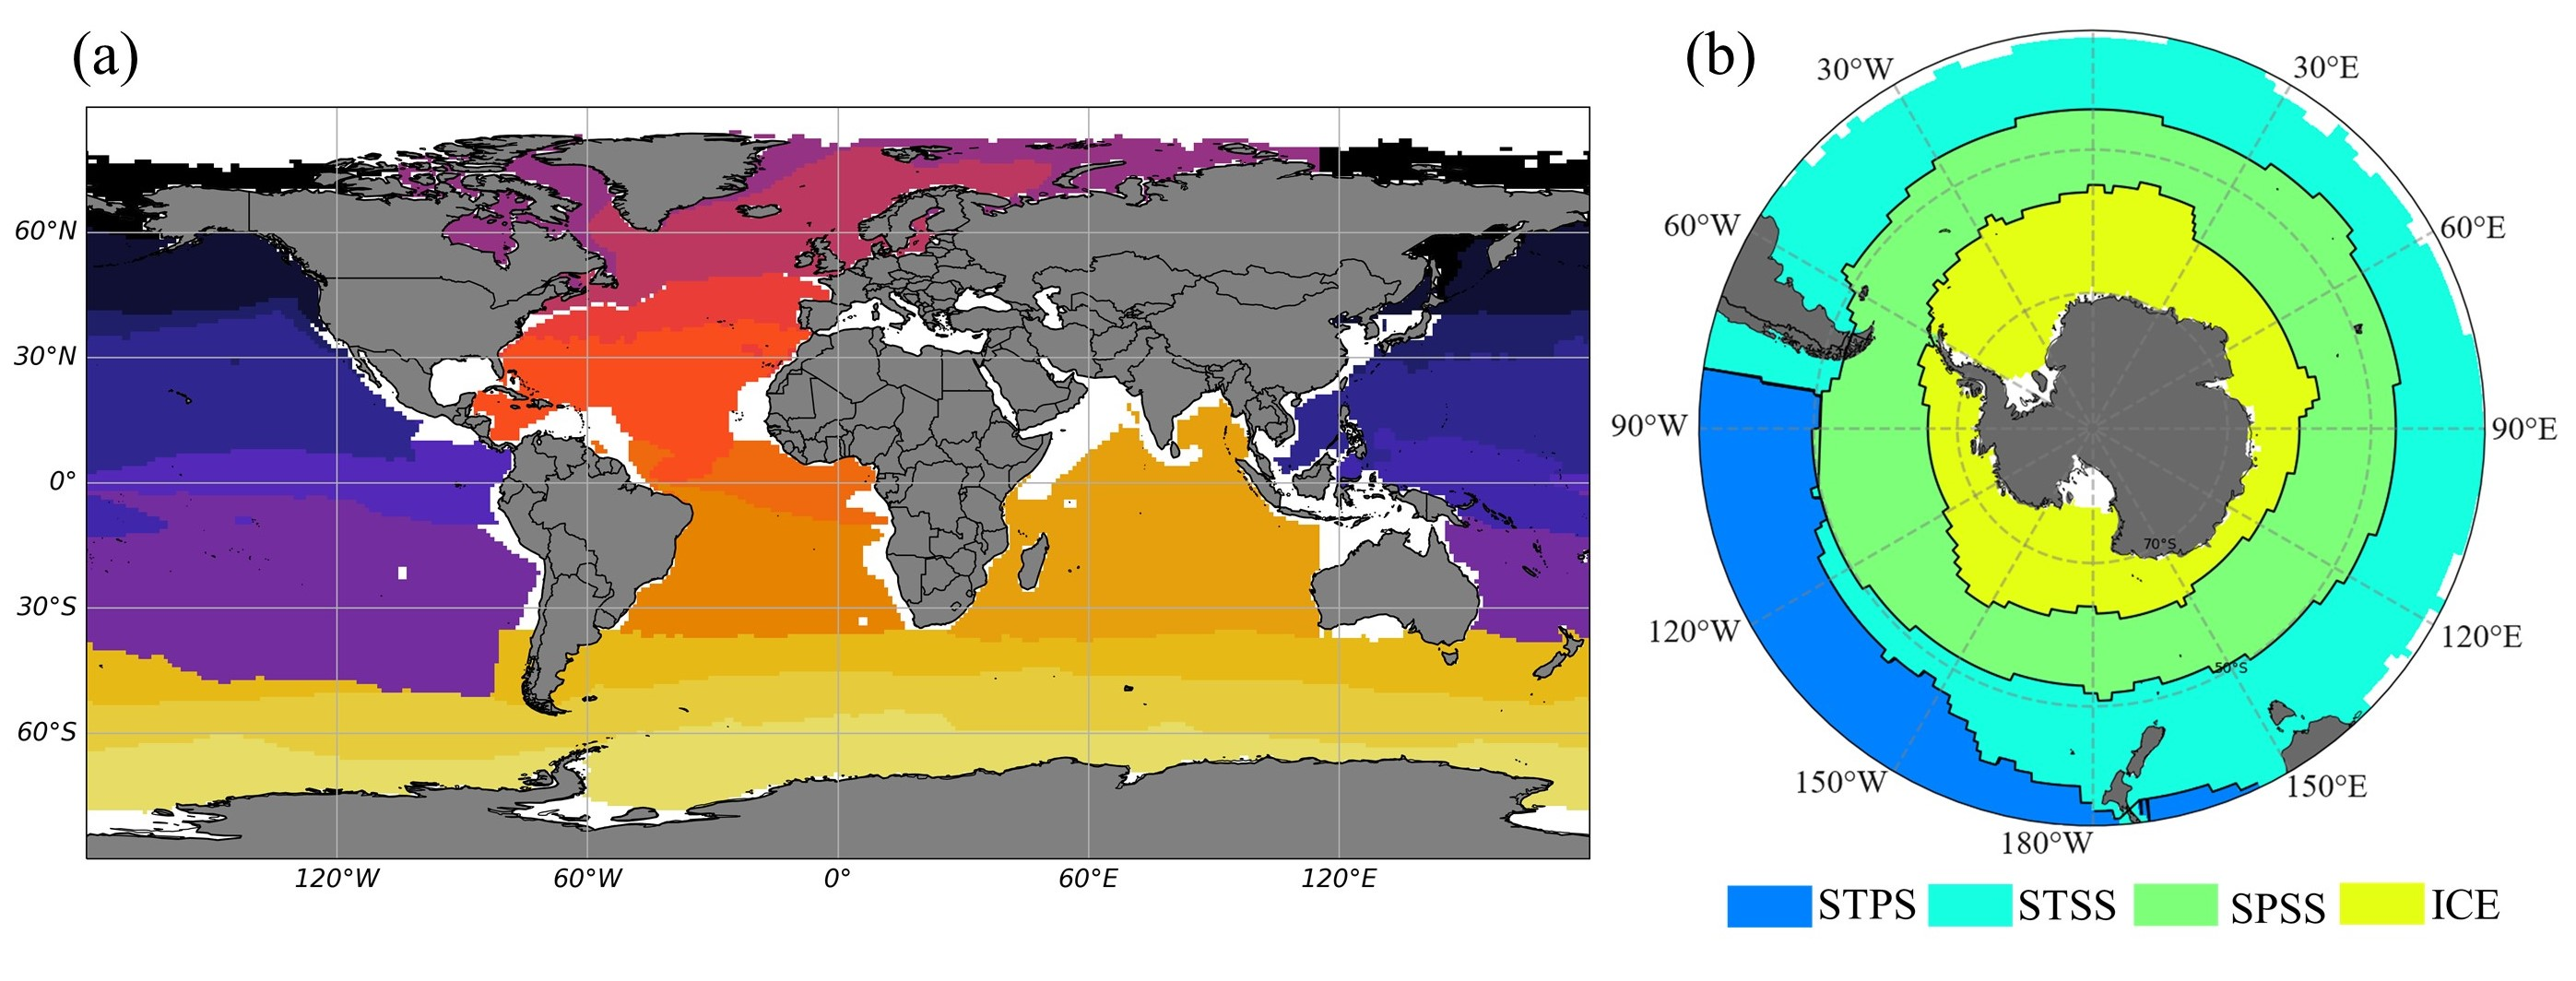
\includegraphics[width=\linewidth]{figure/第二章用图/图2.2-生物分区.jpg}
    \bicaption{\label{fig:生物分区} (a) Fay等人\cite{fay2014global}提出的生物群落全球分区示意图;(b) Fay等人\cite{fay2014global}提出的生物群落南大洋分区示意图}{
    (a) Schematic diagram of global biomes map proposed by Fay et al.\cite{fay2014global};
(b) Schematic diagram of Southern Ocean biomes map proposed by Fay et al.\cite{fay2014global}
    }
\end{figure}

Fay等人\cite{fay2014global}运用多种参数,如海表面温度(SST)、春夏叶绿素a(Chl-a)浓度、冰浓度以及最大混合层深度(MLD)等,对全球的海洋生物群落进行了分类,如图(1)所示,为全球生物群落划分,不同颜色代表了不同的生物群落区。在研究区域被大致划分为四个主要的生物群落:亚热带永久分层生物群系(subtropical permanently stratified biome, STPS)、亚热带季节性分层生物群系(subtropical seasonally stratified biome,STSS)、亚极地季节性分层生物群系( subpolar seasonally stratified biome, SPSS)和冰层生物群系(ice biome, ICE)。这四个群落各自代表了南大洋中不同的生态区域,每个生态区域都有其独特的生物化学特性。划分条件详见\autoref{tab:biomes分区表}。

南大洋的碳汇变化存在较大的争议,主要原因是南大洋的数据不足和遥感数据的冬季缺失。另外,冬季的被动遥感数据受到太阳天顶角、云层和冰的影响,不能发挥最大的观测能力,其中MODIS卫星叶绿素数据在SPSS和ICE区域存在数据缺失,而STSS和STPS区域的数据覆盖率相对较高。对于ICE区域,由于冬季冰层覆盖率较高,碳汇交换受到限制;而SPSS区域,几乎占据了整个南大洋一半的面积,该区域的碳汇变化趋势存在较大不确定性。基于MODIS卫星Chl-a覆盖情况以及各个区域特征,在本文中我们将STSS和STPS区域视为低纬度区域,将SPSS和ICE区域视为高纬度区域进行分析对比。

\begin{table}[htbp]
\bicaption{\label{tab:biomes分区表}Fay等人\cite{fay2014global}划分生物群落的标准}{Fay et al.\cite{fay2014global} Criteria for classifying biomes}
\begin{tabularx}{\textwidth}{XXXXX}
\toprule
Biomes & SST(°C) & Chl-a(mg\ m$^{-3}$) & Max MLD(m) & 备注 \\
\midrule
STPS   & x\textgreater{}=8 & x\textless{}0.25 & x\textless{}=150 & \\
STSS   & x\textgreater{}=8 & x\textgreater{}=0.16 & x\textgreater{}150 &  Chl-a 或 max MLD \\
SPSS   & x\textless{}8     & & & \\
ICE    & & & & 海冰浓度\textgreater{}=0.5 \\
\bottomrule
\end{tabularx}
\end{table}

\section{数据介绍与处理}
\subsection{\texorpdfstring{$p\mathrm{CO_2}$}{}实测数据介绍与处理}
\subsubsection{实测数据介绍}
\begin{figure}[htbp]
    \centering
    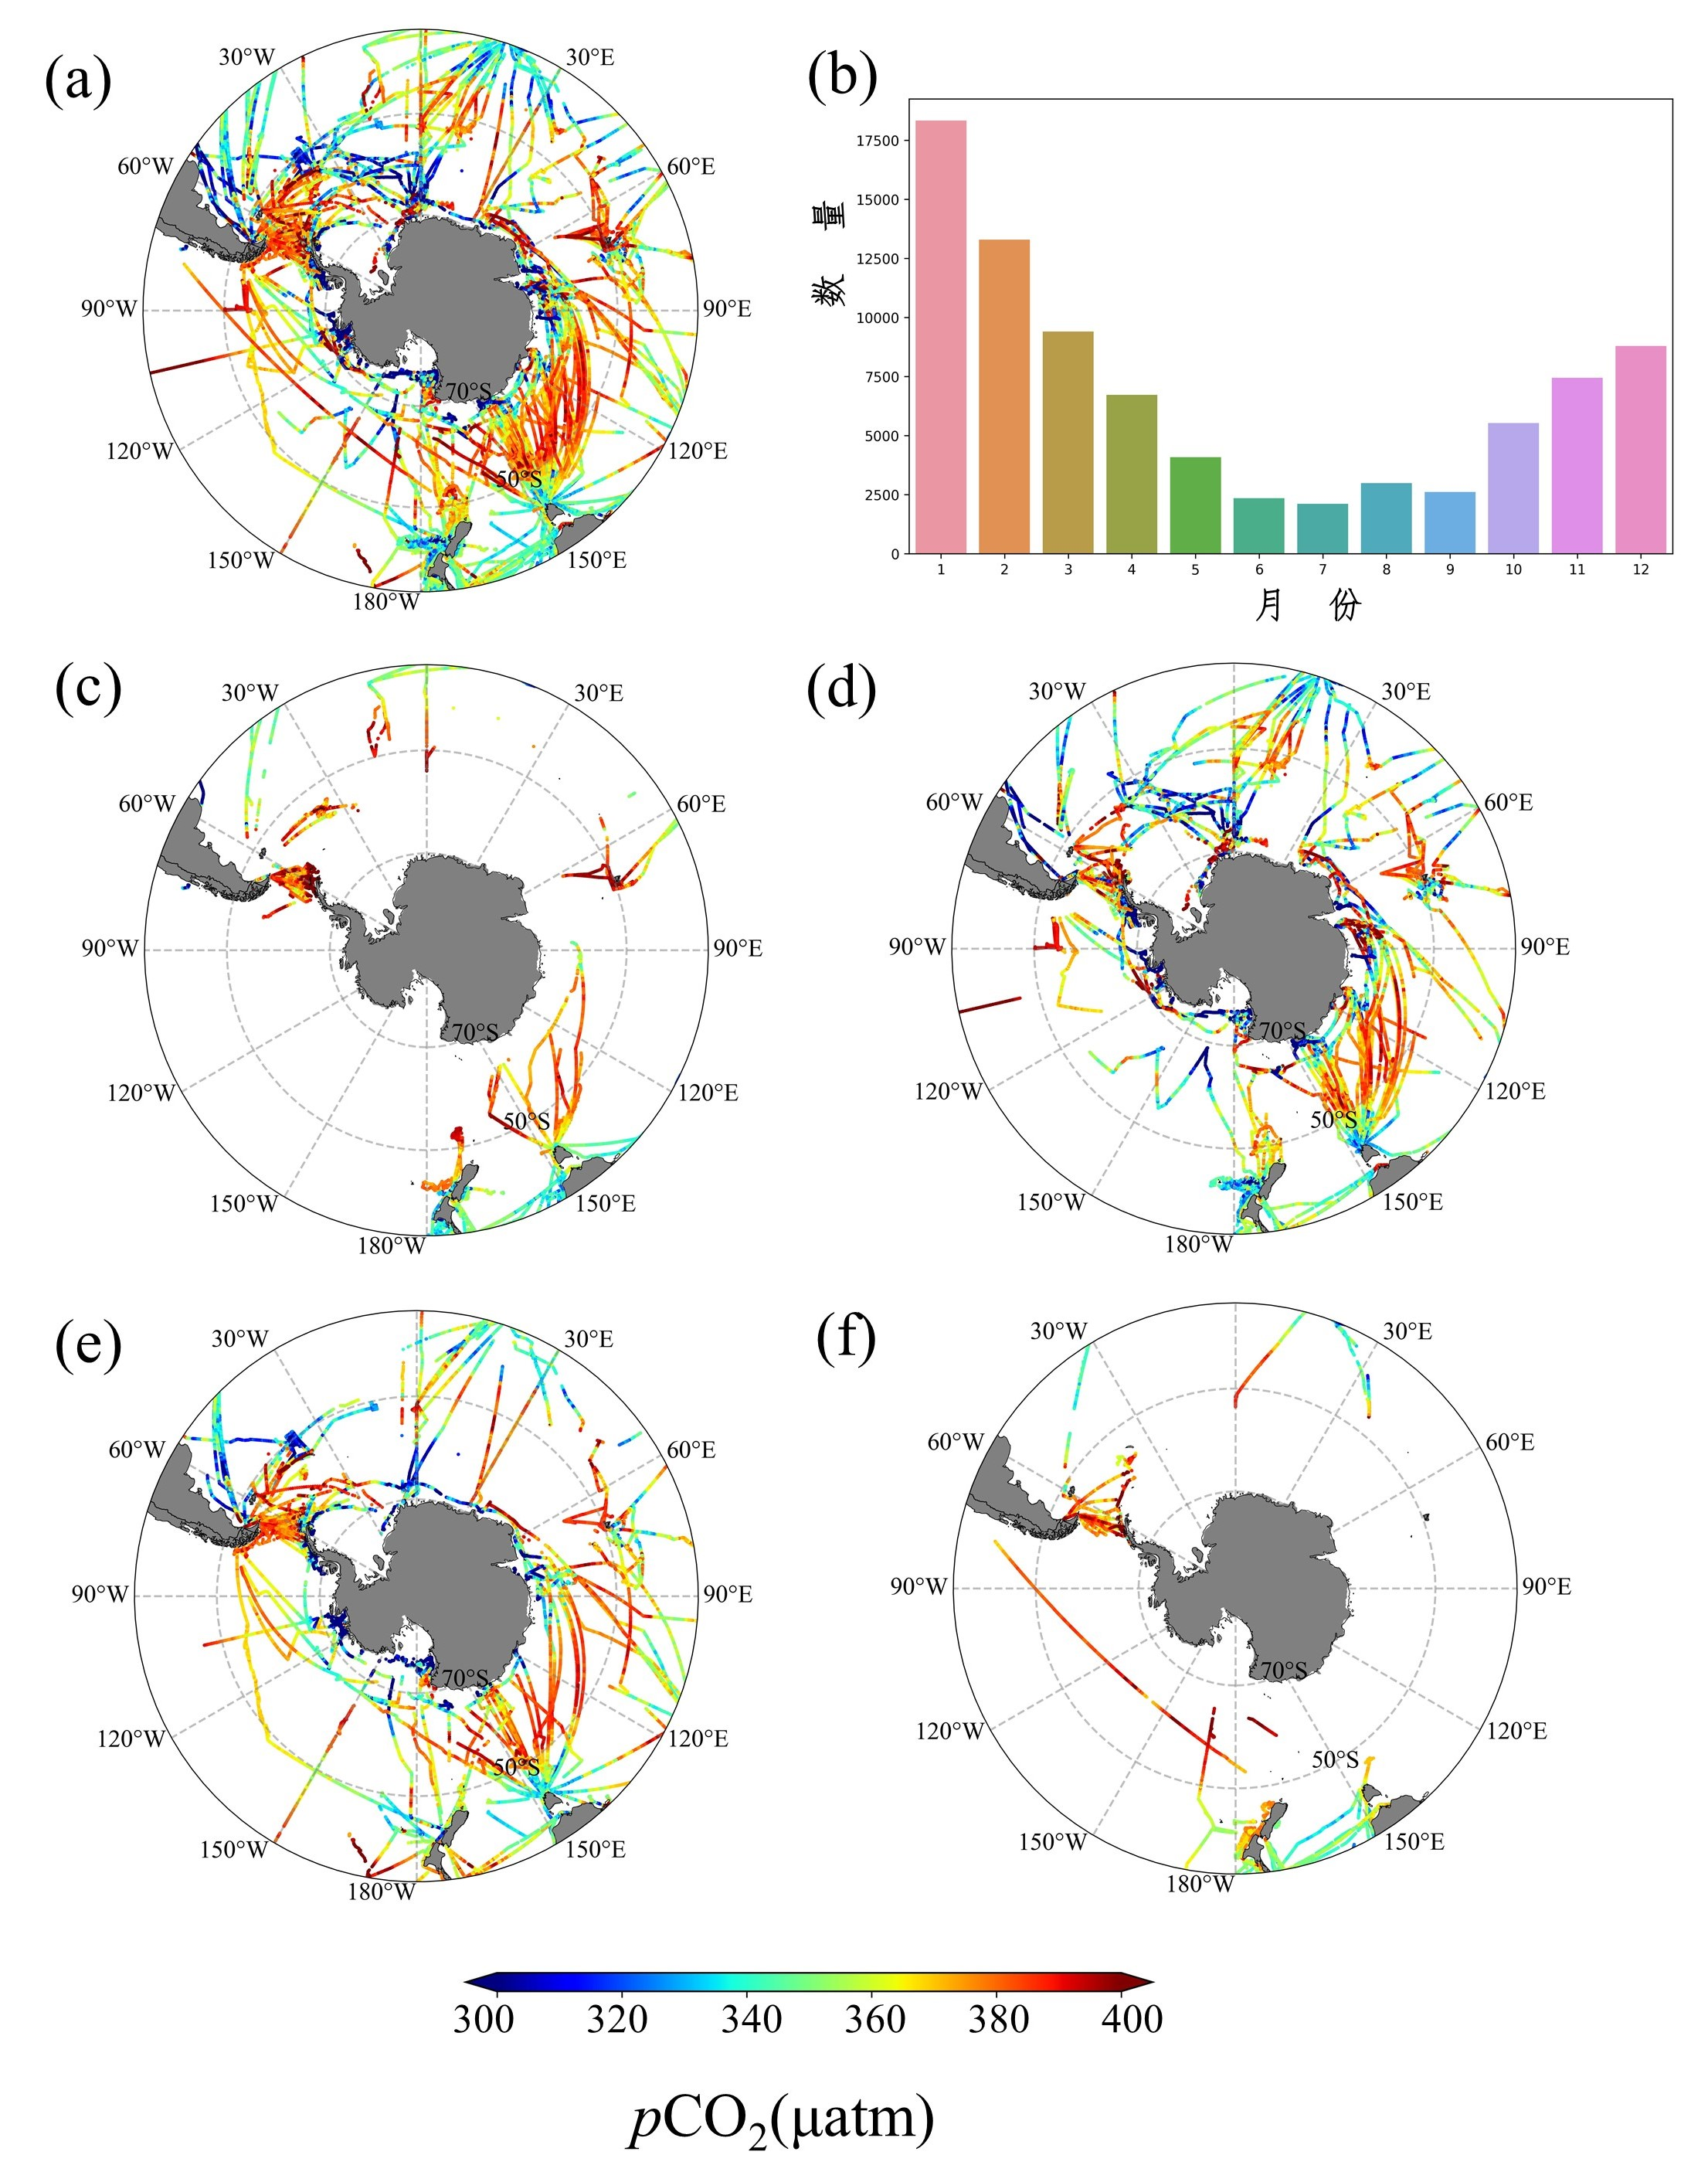
\includegraphics[width=\linewidth]{figure/第二章用图/SOCAT分布图.jpg}
    \bicaption{\label{fig:SOCAT分布} (a)南大洋实测数据(2008.01-2016.12)分布图;(b) 不同月份$p\mathrm{CO_2}$实测数据统计图;(c)(d)(e)(f)分别为南大洋春(8,9,10)、夏(11,12,1)、秋(2,3,4)、冬(5,6,7)四个季节实测$p\mathrm{CO_2}$分布图}{(a) Distribution Map of Observed Data in the Southern Ocean (2008.01-2016.12);
(b) Statistical Chart of Observed $p\mathrm{CO_2}$ Data in Different Months;
(c), (d), (e), (f) are respectively the distribution maps of observed $p\mathrm{CO_2}$ in the Southern Ocean during spring (8, 9, 10), summer (11, 12, 1), autumn (2, 3, 4), and winter (5, 6, 7).}
\end{figure}

在本次研究中,我们选择的实测走航$p\rm CO_2$数据来源于海表$\rm CO_2$地图集(The Surface Ocean $\rm CO_2$ Atlas, SOCAT V 2023, \url{https://socat.info/})\cite{socat2016}。这是一个包含来自十多个国家的船舶、系泊和自主水面测量仪器的二氧化碳溢度(sea surface fugacity of $\rm CO_2$,$f\rm CO_2$)实测数据集,SOCAT v2023版本包含了1957至2023年间全球海洋和沿海海域的3560万次观测和720万次传感器观测数据,其中南大洋区域约有745万条数据记录。该数据集对测量结果进行了质量控制,SOCAT v2023版本中的3560万次$f\rm CO_2$测量精度优于5μatm,$f\rm CO_2$传感器数据精度为5至10μatm。\cite{socat2016} 

该数据集的$f\rm CO_2$测量值以及合成产品是衡量海洋吸收$\rm CO_2$量的关键,为我们了解气候变化以及制定政策提供了重要的信息,已经在$p\rm CO_2$领域的研究中多次被使用\cite{CSIR_ML6,MPI_SOMFFN}。其在研究区间的分布如\autoref{fig:SOCAT分布}-(a)所示,走航数据基本覆盖了整个研究区域。但仍有不足之处,如\autoref{fig:SOCAT分布}-(b)所示,其数量分布存在明显的季节差异,受航行环境影响,夏秋季节的航次数据较多(\autoref{fig:SOCAT分布}-(d),(e)),而春冬季节的数据较少(\autoref{fig:SOCAT分布}-(c),(f));且空间分布的密度不同,德雷克海峡区域的航次最多,而受到出海成本、条件的限制,60°S以南的海域分布较少。

\subsubsection{实测数据预处理}
% (2)实测数据预处理
SOCAT V2023数据集中给出的$f\rm CO_2$需要通过如下公式转换成$p\rm CO_2$数据:
\begin{equation}
    \label{equ:pCO2}
   p\mathrm{CO_2} = \mathrm{fCO_2} \cdot exp(P_{atm}^{surf} \cdot \frac{B + 2\cdot \delta}{R \cdot T})^{-1}
\end{equation}
公式中,$P_{atm}^{surf}$是海表面大气压,单位为Pa,T是海表面绝对温度,单位为K,R是气体常数,为8.314J/(K·mol),而B和$\delta$是矫正系数,单位为$m^3/mol$,分别通过公式\autoref{equ:B},\autoref{equ:delta}计算得到。
\begin{equation}
    \label{equ:B}
   B= (-1636.75 + 12.0408\cdot T - 3.27957 \times 10^{-2}\cdot T^2 +3.165\times 10^{-5}\cdot T^{3})\times 10^{-6}
\end{equation}

\begin{equation}
    \label{equ:delta}
   \delta = (57.7 - 0.118\cdot T)\times 10^{-6}
\end{equation}

处理过程中,我们只使用了QCflag为A-D的数据,为了防止数据冗余且方便与环境变量数据进行匹配,我们将每条航次分开处理,每条数据根据\autoref{equ:pCO2}计算得到$p\rm CO_2$后,将按照经纬度映射到0.25°×0.25°的网格中,如果网格中的一个像素对应有多条数据记录,则取多条数据的平均值。考虑到南大洋地区环境等条件带来的测量误差以及映射方法中导致相邻像素单元中出差$p\rm CO_2$差距过大的现象,最后使用3×3的网格取平均值进行平滑处理,如\autoref{fig:平滑pCO2}所示,是航次号为:33RO20131223的平滑处理效果。
\begin{figure}[htbp]
    \centering
    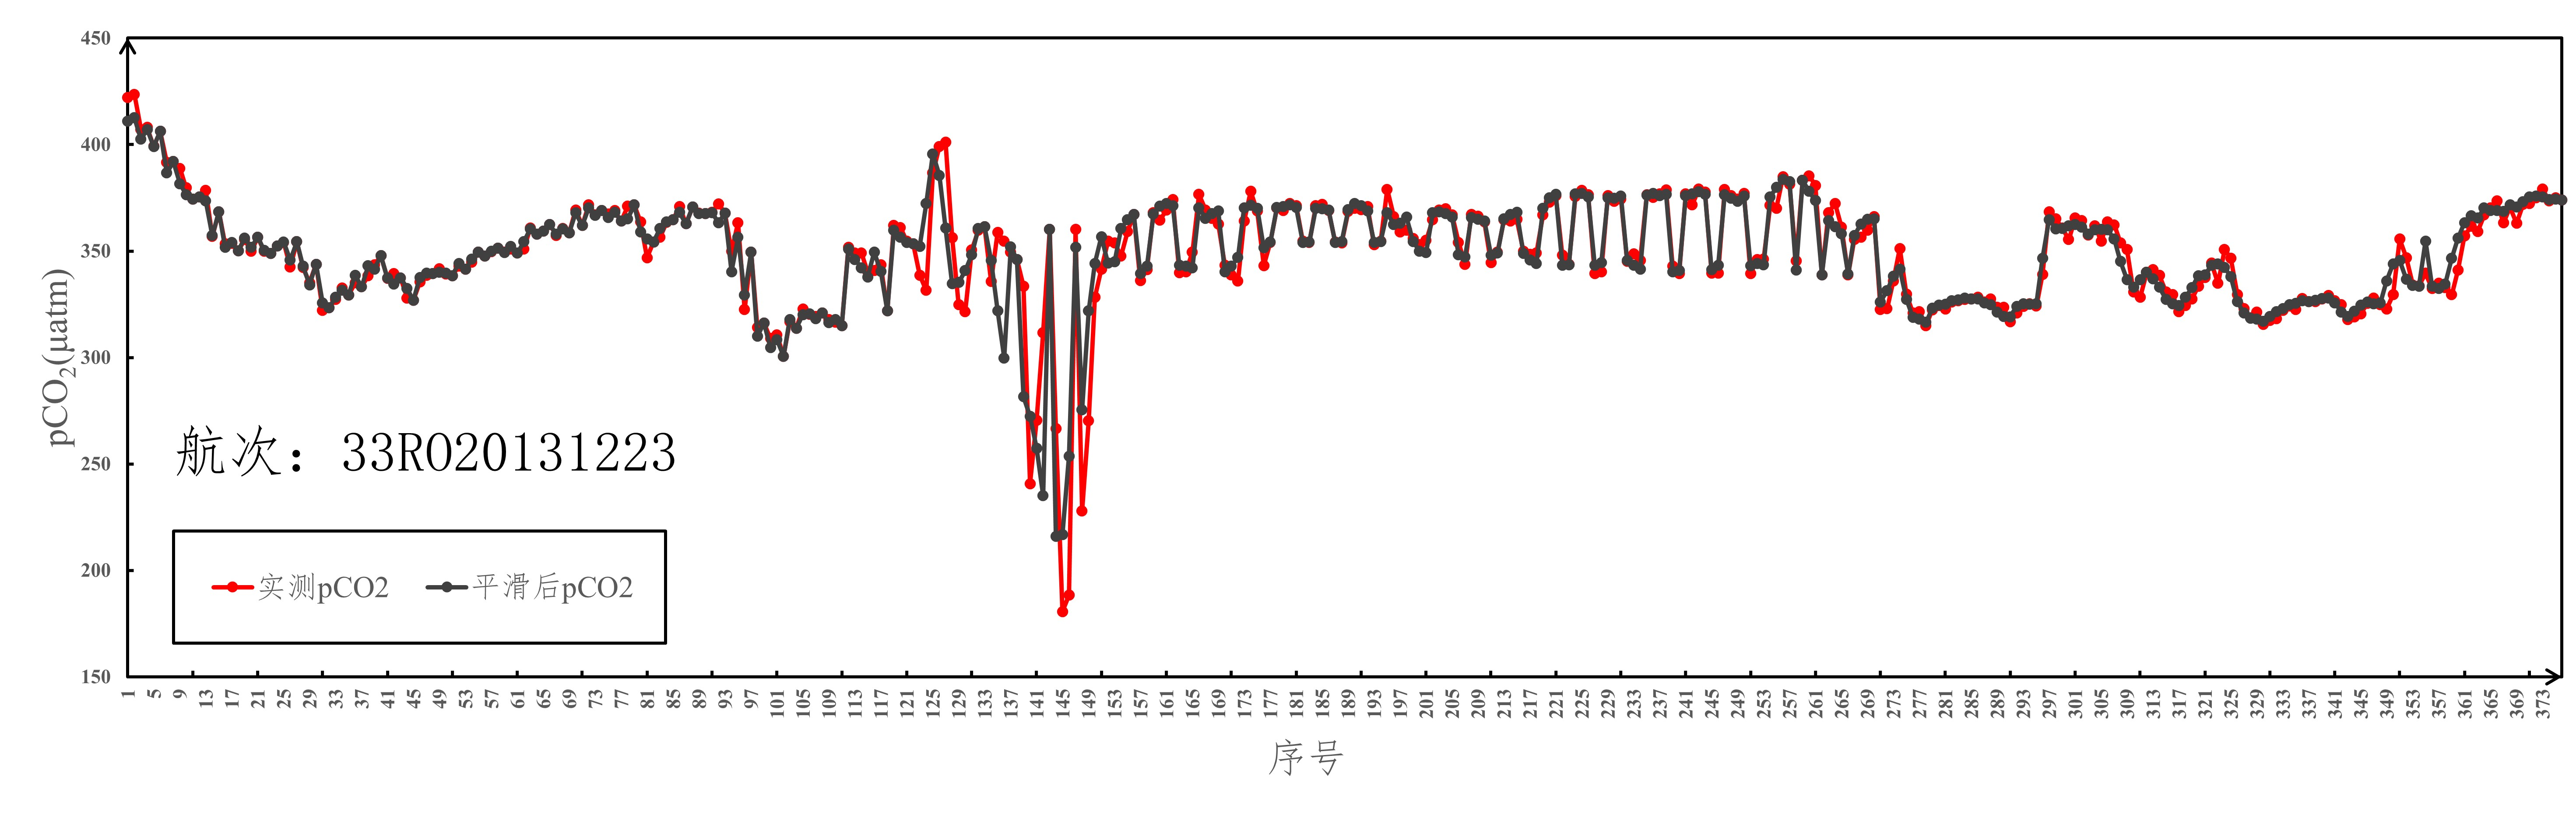
\includegraphics[width=\linewidth]{figure/第二章用图/平滑pCO2.jpg}
    \bicaption{\label{fig:平滑pCO2}航次号为:33RO20131223的平滑处理效果 }{The smoothing effect of the NO. 33RO20131223 cruise}
\end{figure}

% \subsection{遥感数据介绍与处理}
\subsection{CALIPSO卫星介绍与数据处理}
\subsubsection{CALIPSO卫星以及CALIOP传感器介绍}
\begin{figure}[htbp]
    \centering
    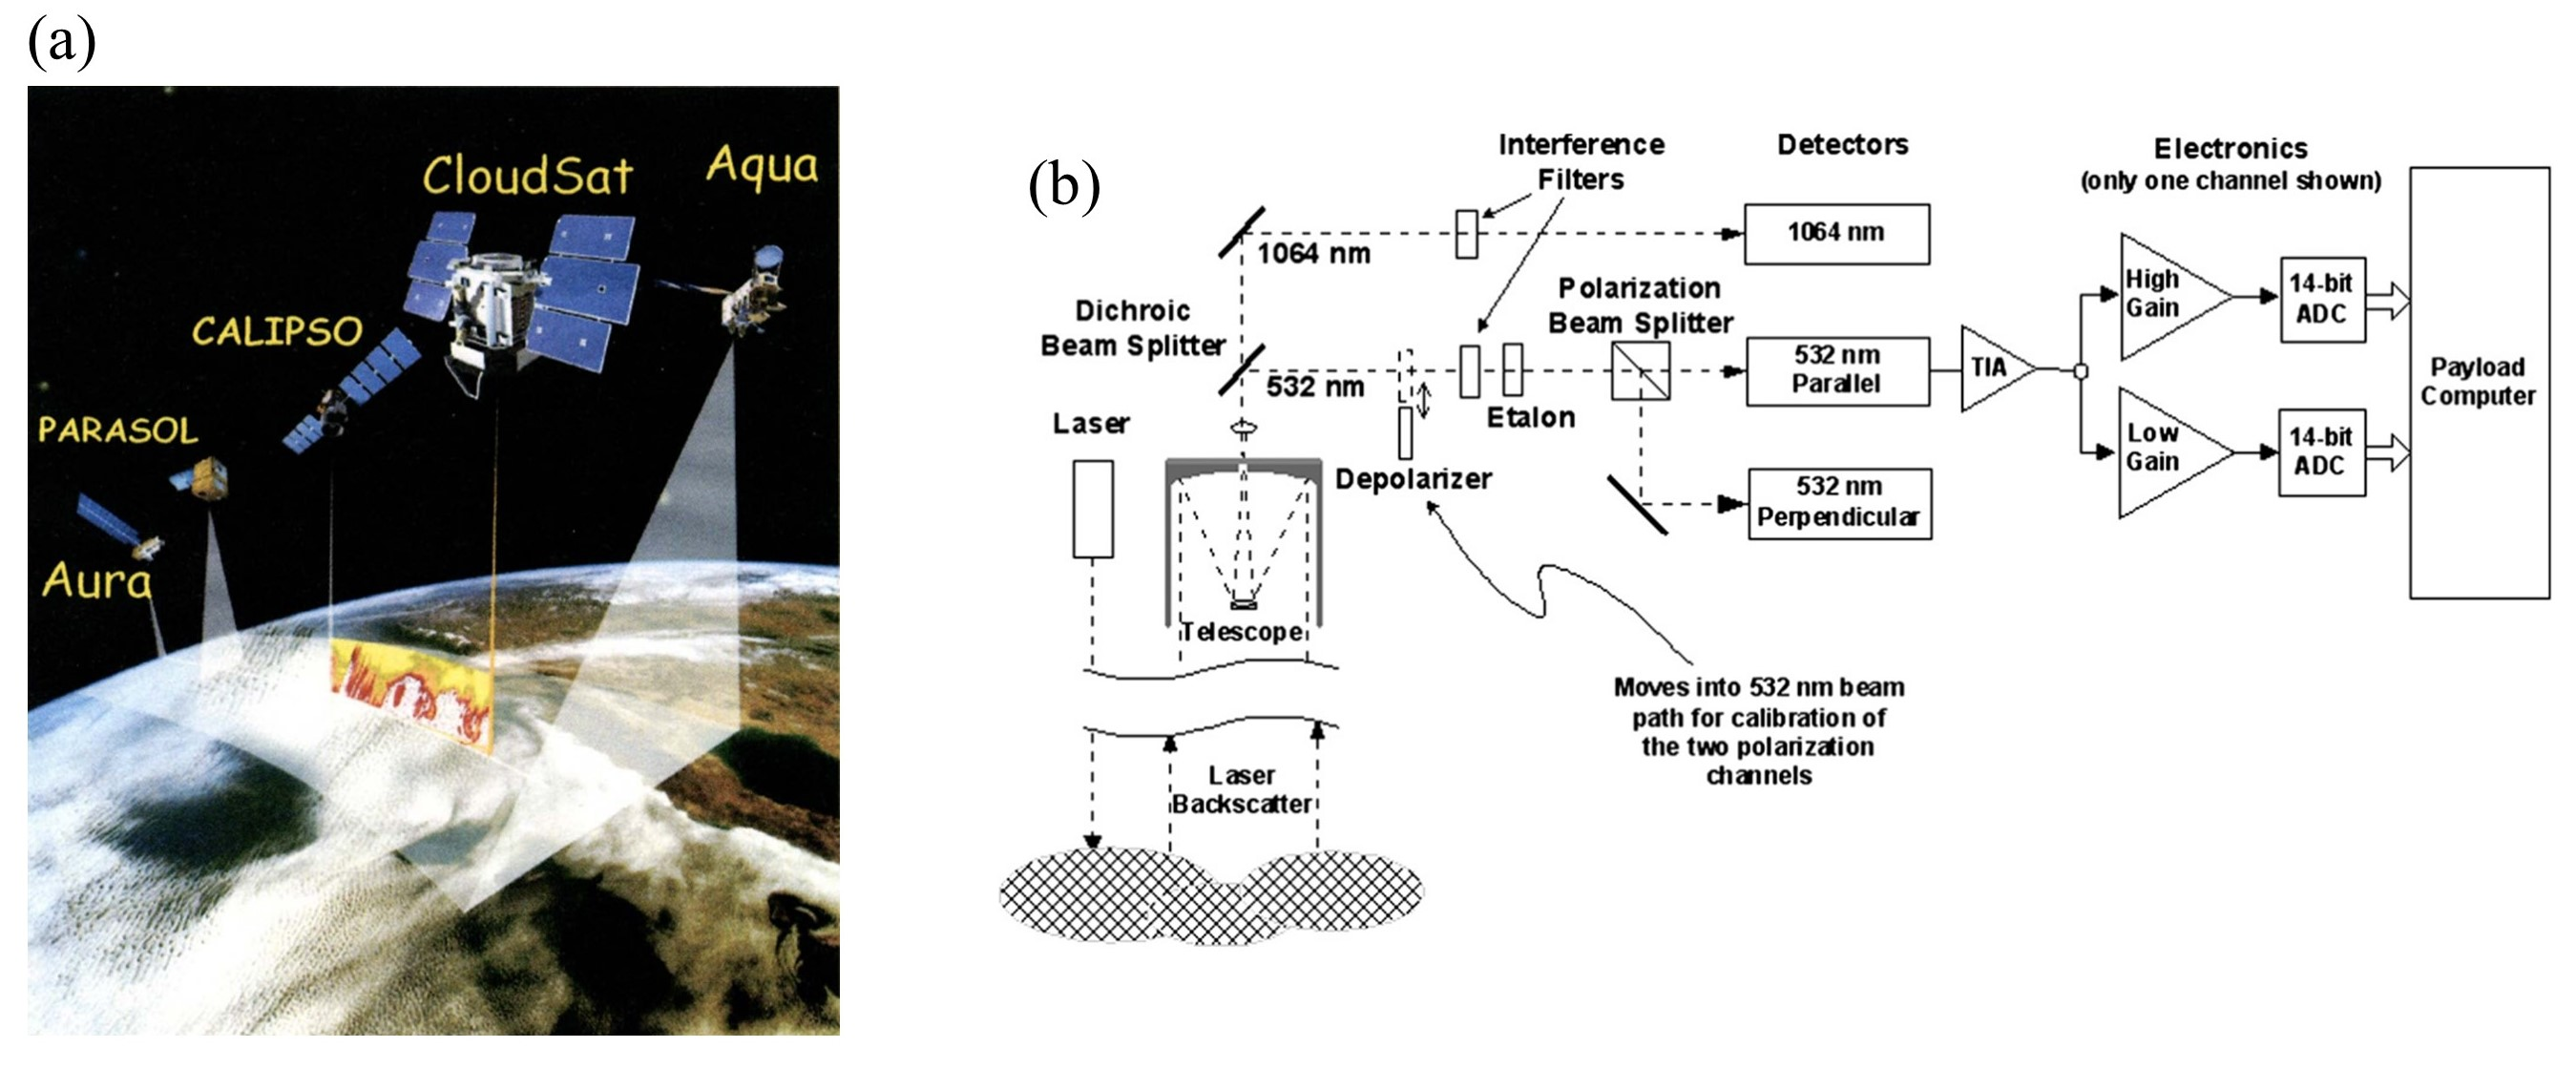
\includegraphics[width=\linewidth]{figure/第二章用图/图2-CALIPSO.jpg}
    \bicaption{\label{fig:CALIPSO卫星} (a) A-train地球观测传感器及其成员\cite{stephens2002cloudsat};(b) CALIOP传感器成像示意图\cite{CALIPSO_2009}}{
    (a) The concept of the A-Train constellation and its members\cite{stephens2002cloudsat};
    (b) Schematic diagram of CALIOP sensor imaging\cite{CALIPSO_2009}
    }
\end{figure}

云气溶胶激光雷达和红外探路卫星观测(the Cloud-Aerosol Lidar and Infrared Pathfinder Satellite Observation, CALIPSO)卫星是由美国国家航空航天局(National Aeronautics and Space Administration, NASA)和法国国家空间研究中心(the Centre National d’Etudes Spatiales, CNES)合作研发\cite{winker2003accounting,CALIPSO_2009}。其作为地球系统科学探路者项目(Earth System Science Pathfinder, ESSP)的一部分,于2006年发射,是A-train地球观测传感器套件的一部分(如\autoref{fig:CALIPSO卫星}-(a)),其目标是填补我们在观测气溶胶和云层全球分布和特性方面的现有空白。\cite{CALIPSO_2009,winker2003accounting}A-train系列卫星在705公里的太阳同步极地轨道上,绕行周期为16天,在每日当地时间约01:30和13:30分别过境一次,轨道间距大约为1.55°,轨道倾角为98.2°,提供了82°N到82°S的全球覆盖。\cite{stephens2002cloudsat,CALIPSO_2009}

CALIPSO卫星上携带的主要仪器是云—气溶胶正交偏振激光雷达(the Cloud-Aerosol Lidar with Orthogonal Polarization, CALIOP),是第一个提供全球大气测量的偏振激光雷达,为科学界提供了新的观测能力。CALIOP是一种双波长偏振激光雷达,拥有波长为532nm和1064nm两个通道(如\autoref{fig:CALIPSO卫星}-(b)),能够不间断地收集82°N和82°S之间气溶胶和云在两个波段上的衰减散射以及波长532nm极化后向散射。\cite{CALIPSO_2009}同时它在大气中的垂直采样率为30m,但是由于532nm波段在水中的折射率增加了1.32倍,因此垂直采样分辨率降低到22.5m。它在大气中的垂直采样频率为30m,但由于532nm波段在水中的折射率增加了1.32倍,因此垂直采样分辨率被调整到22.5m。CALIPSO还配备了两种被动传感器:一是宽视场相机,这是一种基于电荷耦合器件的可见光传感器,其在距离卫星下方2.5公里的范围内的像素空间分辨率为125米,在两侧延伸至30公里的带状区域内,其余像素的空间分辨率为1000米。二是红外成像辐射计,它是一种三通道设备,其空间分辨率为1公里,波段为61公里。这两种传感器都以激光雷达的足迹为中心,为我们提供了周边大气的视图。

相较而言,CALIOP激光雷达具有无可比拟的优势。它可以发射自己的激光,无需受太阳光的限制,能在白天和黑夜都能工作。此外,雷达是唯一能提供高分辨率的气溶胶剖面的技术,即使在明亮的地表如荒漠、雪层或明亮的云层上,也能实现气溶胶的观测。激光雷达能穿透高亮的薄云层,绘制出大气的大部分轮廓。还可以通过测量后向散射的去极化信号,提供垂直分辨率的冰水相位测量\cite{CALIPSO_2009,winker2003accounting}。因此,它在弥补被动遥感的缺陷方面具有优势,即使在冬季极地地区也能发挥重要作用。

\subsubsection{CALIPSO卫星数据及处理}
\begin{figure}[htbp]
    \centering
    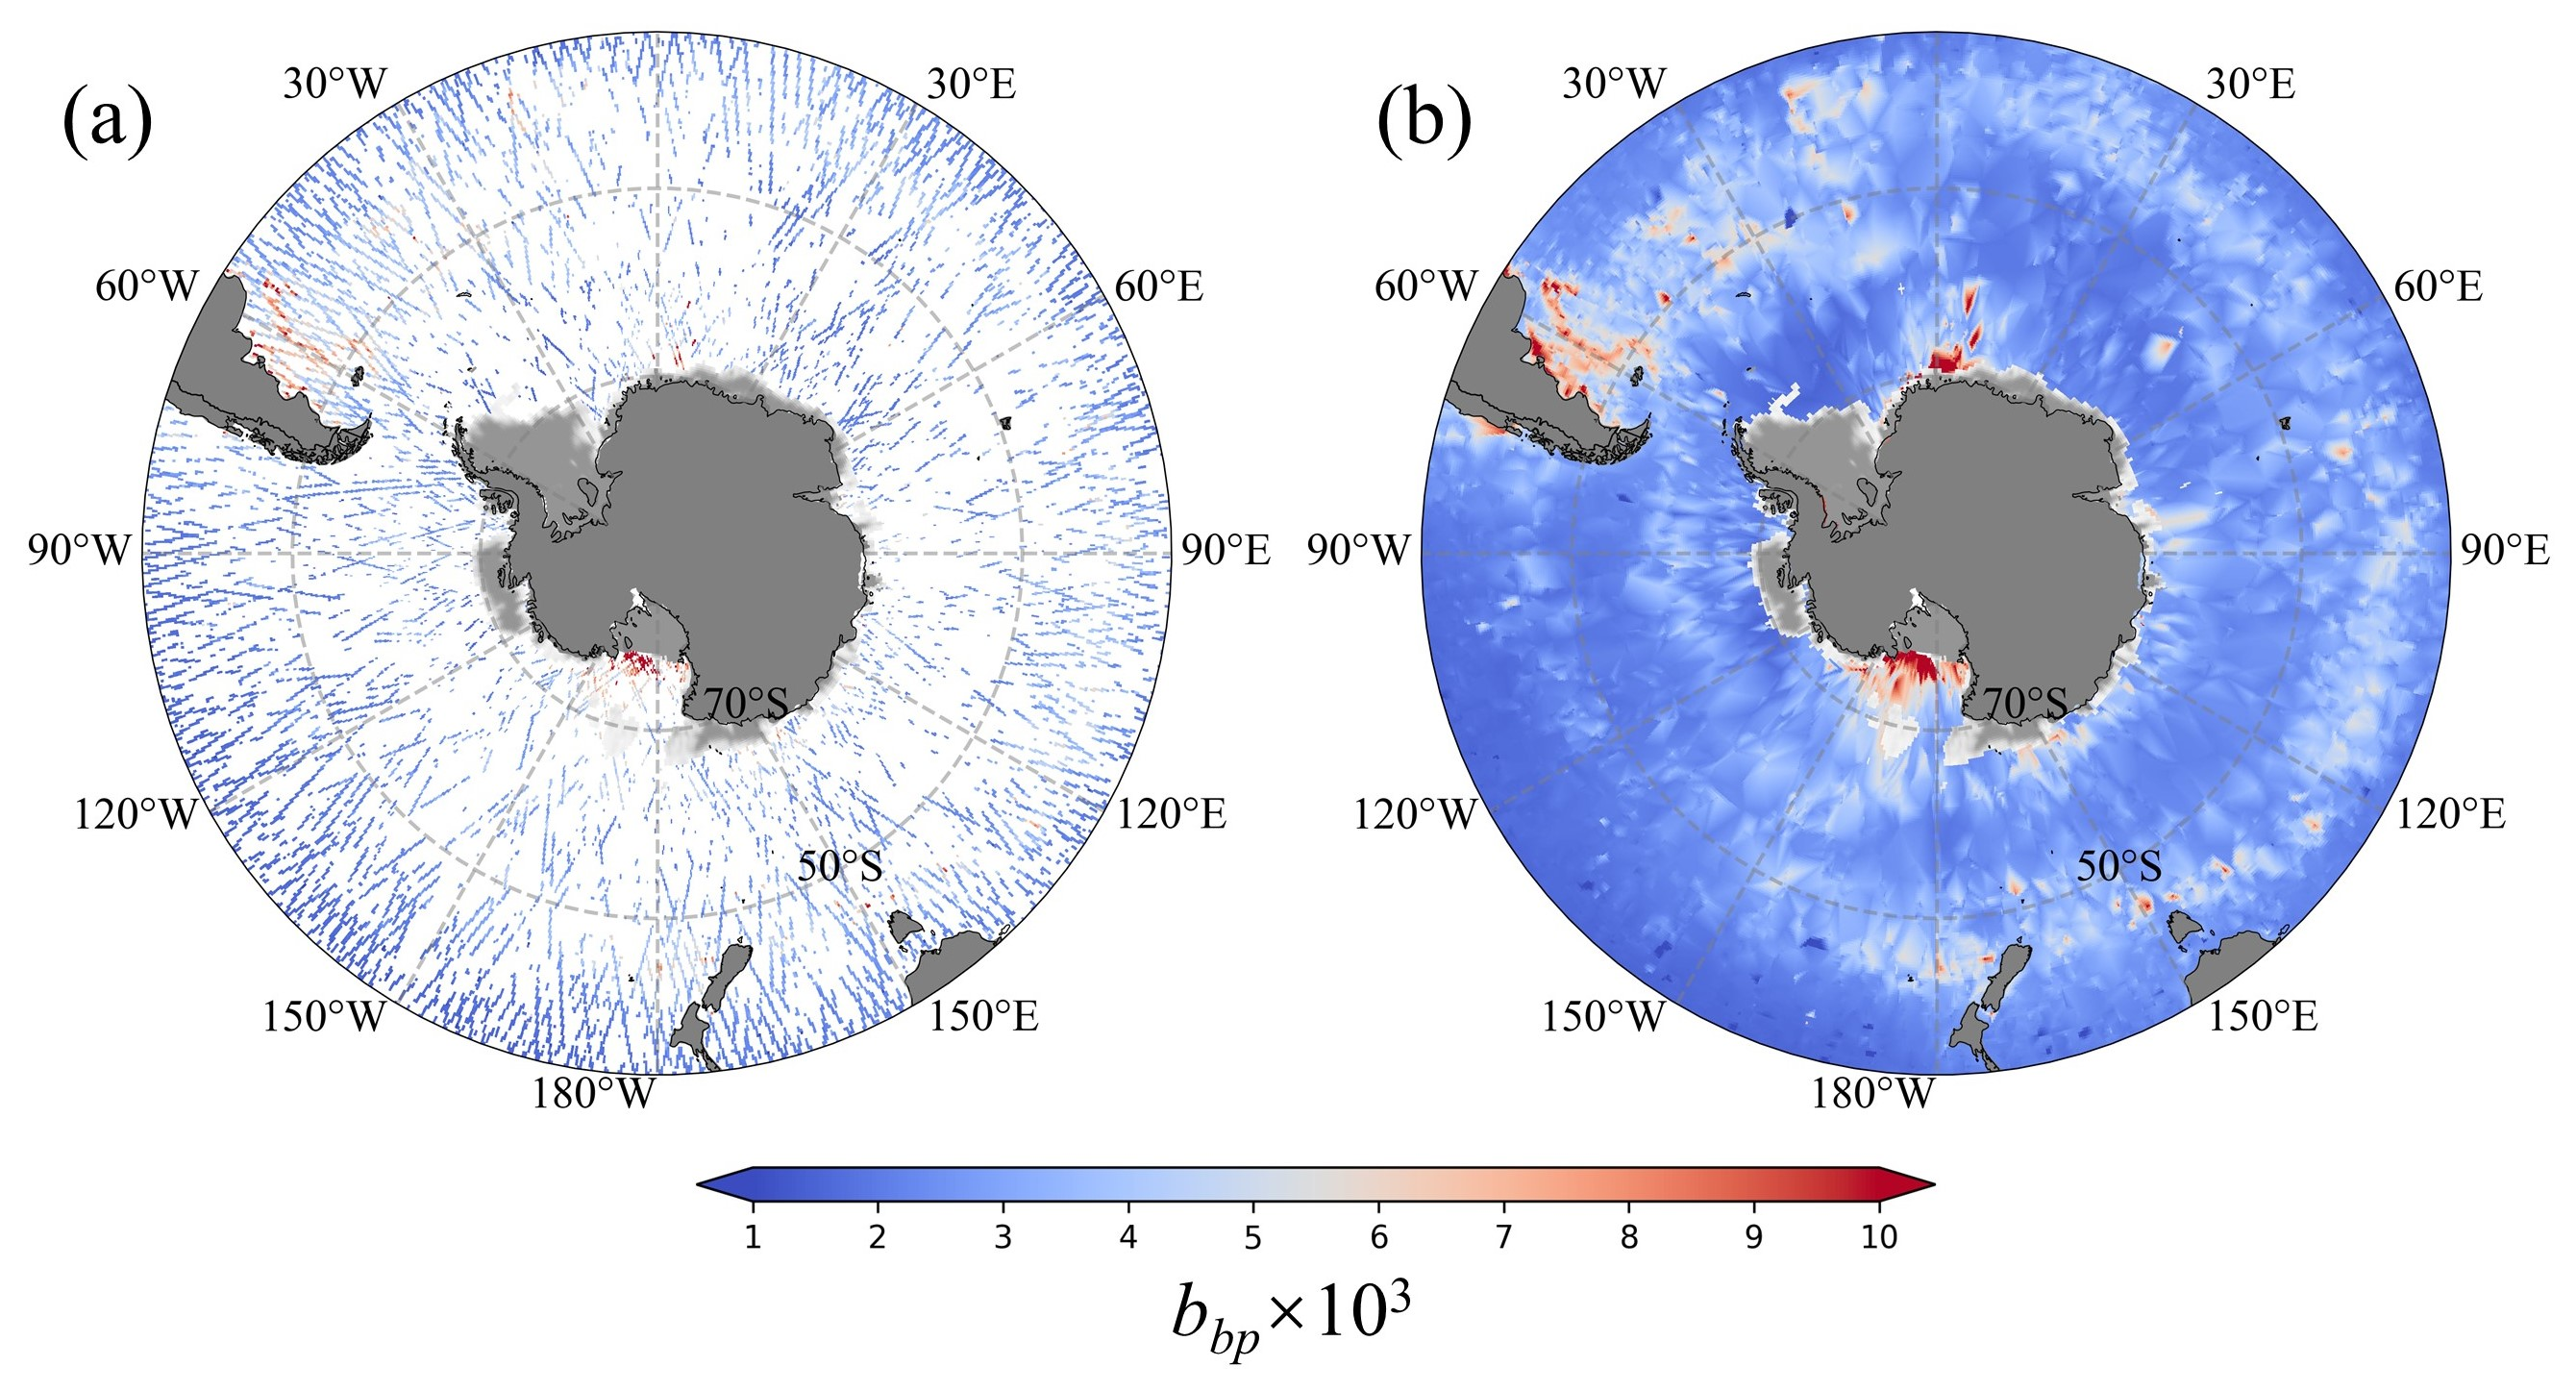
\includegraphics[width=\linewidth]{figure/第二章用图/图2-bbp处理.jpg}
    \bicaption{\label{fig:bbp处理} (a) 原始$b_{bp}$数据分布图(2011年2月);(b) 二维线性插值后得到的$b_{bp}$分布图}{
    (a) Distribution plot of raw $b_{bp}$ data (February 2011);
    (b) Distribution plot of $b_{bp}$ data after 2D linear interpolation
    }
\end{figure}

颗粒后向散射系数(subsurface particulate backscatter coefficients, $b_{bp}$)描述颗粒在受到入射光线激发后向相反方向散射的强度,其对于了解海洋生态具有重要作用。由于海表面反射的信号污染,从CALIOP获取$b_{bp}$数据具有一定的挑战性,但CALIOP的交叉极化通道测量到的信号几乎完全是由于颗粒物质的反向散射,Berenfired等人\cite{2013Space}基于海表以下柱积分下通量后向散射的交叉极化分量$\beta _ w$来反演得到$b_{bp}$值,且与现场评估的结果表明了基于CALIOP计算得到的$b_{bp}$值的正确性。

$b_{bp}$数据主要来自于CALIOP的532nm极化波长,其提供了白天和夜间观测的数据(\url{http://orca.science.oregonstate.edu/lidar_nature_2019.php})\cite{behrenfeld2019global},本文中使用了白天和夜间的数据,考虑到数据量的大小以及最后插值的效果,我们将$b_{bp}$白天和夜间观测得到的数据进行合并,然后按照年月平均到一个0.25°×0.25°的网格中,若同个网格中个一个像素若有多个值则计算平均值,接着使用二维线性插值的方法来填补上少量的观测空白区域,如\autoref{fig:bbp处理}所示,(a)图为2011年2月观测数据平均后的结果,(b)图为使用插值方法填充得到的$b_{bp}$分布图。按照此方法最终获取到2008年-2016年每月的0.25°×0.25°$b_{bp}$插值结果。

\subsection{MODIS 卫星遥感数据}
中等分辨率成像光谱仪(Moderate Resolution Imaging Spectroradiometer, MODIS)是搭载在美国对地卫星(Earth Observation System, EOS)系列卫星 Terra 和 Aqua 卫星上的传感器。这两颗太阳同步极轨卫星于 2002 年 5 月发射,是EOS中用于观测全球生物和物理过程的重要工具。TERRA卫星于1999年12月18日发射成功,为上午星,从北向南于地方时10:30左右通过赤道。而AQUA卫星于2002年5月4日发射成功,为下午星,从南向北于地方时13:30左右通过赤道。这两颗卫星相互配合,每1\~2天可重复观测整个地球表面,获取丰富的数据。MODIS传感器数据获取快且覆盖范围广,如\autoref{tab:MODIS卫星波段},光谱范围从0.4微米(可见光)到14.4微米(热红外),实现全光谱覆盖。其能够提供36个波段的观测数据,如表所示,其中的 7 个波段被广泛且较为频繁地应用于海洋水色遥感,比如叶绿素、悬浮物等。其数据空间分辨率为250m~1000m,扫描宽度达2330公里。

\begin{table}[htbp]  
\centering % 居中表格  
\bicaption{\label{tab:MODIS卫星波段}MODIS卫星波段设置}{the Settings of MODIS satellite band}
\begin{tabularx}{\textwidth}{>{\centering\arraybackslash}p{1cm}>{\centering\arraybackslash}p{1.7cm}>{\centering\arraybackslash}p{1.7cm}*{3}{>{\centering\arraybackslash}X}}
 % \textwidth让表格宽度等于页面宽度*,{6}{X}表示6列,每列都是X类型(可伸缩)  
\toprule % 使用booktabs包提供的更好看的表头线条  
波段 & 波段范围 & 中心波长 & 波段宽度 & 饱和辐亮度 & 主要应用 \\   
\midrule % 使用booktabs包提供的表身线条  
8 & 204--420 & 412 & 15 & 44.9 & 叶绿素 \\  
9 & 438--448 & 443 & 15 & 41.9 & 叶绿素最大吸收 \\  
10 & 483--493 & 488 & 10 & 32.1 & 叶绿素其他色素 \\  
11 & 526--536 & 531 & 10 & 27.9 & 叶绿素 \\  
12 & 546--556 & 551 & 10 & 21.0 & 叶绿素、悬浮物 \\  
13 & 662--672 & 667 & 10 & 9.5 & 沉淀物、大气层 \\  
14 & 673--683 & 678 & 10 & 8.7 & 大气校正、荧光基线 \\   
\bottomrule % 使用booktabs包提供的表尾线条  
\end{tabularx}  
\end{table}  

海表面温度(Sea Surface Temperature, SST)与$p\mathrm{CO_2}$之间有着十分紧密的联系,一般来说,SST升高会会加大$\mathrm{CO_2}$在水中的溶解度,会致使更多的$\mathrm{CO_2}$溶于海水中。当然,任何一个变量变化都会引起其他环境变量的变化,比如SST的升高会影响水中的生物活动,从而改变$p\mathrm{CO_2}$浓度。本研究中使用到的SST数据来自于美 国 国 家 航 空 航 天 局 (National Aeronautics and Space Administration, NASA) 海 洋 水 色 处 理 中 心 (Goddard Space Flight Center, GSFC, \url{http://oceancolor.gsfc.nasa.gov/}),是来自于MODIS遥感L3级月平均、8天平均数据产品,空间分辨率为 4 km×4 km (0.0416°×0.0416°)的等距柱面圆柱投影栅格数据。另外,SOCAT数据集中也提供了SST的实测数据以供使用。

叶绿素a浓度数据(chlorophyll-a concentration, Chl-a)作为表征生物过程对$p\mathrm{CO_2}$影响的变量,在多数研究中已被证明占有主导地位\cite{brown2019enhanced,tu2021increase}。其作为植物进行光合作用的关键色素,其浓度能够反映水生生物,特别是浮游植物的生长状况,因此在叶绿素浓度较高的区域,通常会发现$p\mathrm{CO_2}$的浓度相对较低。本研究中主要使用到的Chl-a数据与SST一样来自于MODIS卫星数据L3级月平均产品。

\subsection{混合层深度数据}
海水混合层深度(Mixed Layer Depth, MLD)是指海洋上层密度相对比较均匀的海水深度,混合层主要是由辐射、风力搅拌、降水等大气场强迫作用造成的海水对流混合,从而形成了在垂直方向上温度、盐度、密度近似均匀的分布。MLD与$p\mathrm{CO_2}$之间存在复杂的关系,首先,MLD决定了海表面与大气之间气体交换能力的强弱,其次,MLD能够反映出海洋动力过程的强弱,此外,MLD还受到季节、气候等多种因素的影响,这与$p\mathrm{CO_2}$变化也有一定的联系。

本研究中所使用到的MLD来自于美国全球海洋数据同化实验室中建立的混合坐标海洋模型(HYbrid Coordinate Ocean Model, HYCOM, \url{https://hycom.org/})中的海水混合层深度(\url{http://www.science.oregonstate.edu/ocean.productivity/}),它是根据HYCOM中的温度、盐度和压强等变量计算出的,其提供了1997-2022年间的、空间分辨率为0.082°×0.082°(9Km)、8天和月平均时间分辨率的MLD数据,在该数据集中,MLD定义为大于表层海水密度0.125Kg m$^{-3}$ 的海水深度。


\subsection{海表面盐度数据}
海表面盐度(Sea Surface Salinity, SSS)会影响海水的密度,当SSS升高时,海水密度会增大,从而影响$\mathrm{CO_2}$在海水中的溶解度,另外,SSS对于海洋生物生存环境也有着至关重要的影响,从而间接地影响$p\mathrm{CO_2}$大小。本文中使用到的SSS数据来自于欧洲哥白尼海洋全球再分析产品(Copernicus Marine Global Reanalysis Product, \url{https://data.marine.copernicus.eu/products})。它是由哥白尼海洋环境监测服务创建的,只在充分了解全球海洋情况,并且提供了1/12°的涡分解的全球海洋模拟。其中的全球海洋物理再分析产品(Global Ocean Physics Reanalysis,\url{https://data.marine.copernicus.eu/product/GLOBAL\_MULTIYEAR\_PHY\_001\_030/description})是基于实时全球预报CMEMS系统,使用了降阶卡尔曼滤波对观测结果进行同化,使用了3D-VAR方法为温度和盐度的大尺度偏差提供校正。本研究中使用了其提供的1993年至今的空间分辨率为0.083° × 0.083°的月平均、日平均SSS数据。


\subsection{海表面风速数据}
海表面风速主要影响海洋表面的动力学过程。在一般情况下,海表面风速的增大可能会促进海水的垂直混合,使得海水中的$\rm CO_2$更容易与大气进行交换。但这种交换过程还会受到海水的温度、盐度等其他因素的影响,因此海表面风速和海表$p\mathrm{CO_2}$之间的关系并不是简单的线性关系。因此,在构建模型时需要将风速纳入考虑范围,以提高模型的准确性和预测能力。

本研究中使用的风速数据来自于CCMP v2(Cross-Calibrated Multi-Platform, \url{https://data.remss.com/ccmp/v02.0/})数据产品,它是一个结合交叉校准的卫星微波风数据和仪器观测数据,并且使用了变分分析方法(Variational Analysis Method, VAM)生成0.25°×0.25°分辨率的月平均三级再分析数据产品。遥感系统(Remote Sensing System, RSS)提供了交叉校准多平台,可以用来下载星载被动和主动微波获取的卫星风速数据,CCMP数据集在亮度温度水平上相互校准,并且使用了应用了准确的海面发射率模型和辐射传输方程来推导海面风以达到校准精度0.2摄氏度以内。其与多个微波辐射计平台(包括SSMI、SSM/I、SSMIS、AMSR、TMI、WindSat和GM等)的风速反演结果高度一致,VAM将RSS仪器数据与系泊浮标测量数据和风场的初始估计相结合,证实了测量结果是一致的,误差在0.8ms$^{-1}$以内。CCMP产品覆盖了南纬79°到北纬79°,且CCMP v2 数据集只提供了1987.1-2019.4时间段内的月平均数据,而2019年4月之后则需要从每日4次的风场数据中计算得出。

\subsection{大气\texorpdfstring{$\mathrm{CO_2}$}{}摩尔分数以及大气\texorpdfstring{$p\mathrm{CO_2}$}{}数据}
大气$p\mathrm{CO_2}$与海表$p\mathrm{CO_2}$大小决定着海水吸收还是排放$\mathrm{CO_2}$,这对海洋碳循环有着十分重要意义。而大气$p\mathrm{CO_2}$可以使用大气中$\mathrm{CO_2}$摩尔分数($x\rm CO_2$)计算出来,它是指在大气中$\mathrm{CO_2}$分子的数量与总气体分子数之比。它通常用于表示大气中$\mathrm{CO_2}$的浓度,本研究中使用的$x\rm CO_2$数据来源于美国国家海洋和大气管理局(National Oceanic and Atmospheric Administration, NOAA)温室气体海洋边界层( Marine Boundary Layer, MBL, \url{https://gml.noaa.gov/ccgg/mbl/})数据库。MBL数据站点通常位于远洋地域,只有盛行的陆上风,而且不包括来自高海拔、受人类活动影响的站点测量结果,其提供了全球$\mathrm{CO_2}$增加的最低噪声表示。

而大气$p\mathrm{CO_2}$可以根据公式计算得出:
$$
p\mathrm{CO_2^{air}} =x\mathrm{CO_2}\times (P_{sea-level}-P_{water}) 
$$

其中,$P_{sea-level}$和$P_{water}$分别为海平面、水蒸气气压,单位均为帕(Pa),本研究中使用到的$P_{sea-level}$数据是来自于NCEP再分析模型II产品(NCEP-DOE Reanalysis 2, \url{https://psl.noaa.gov/data/gridded/data.ncep.reanalysis2.html})。NCEP-DOE数据中使用了最先进的分析-预测系统,并使用了1979-2022年的数据进行数据同化,具有较高的准确性。而$P_{water}$是根据$P_{sea-level}$和SST计算得出。

\subsection{海冰浓度数据}
本研究中使用的海冰浓度数据主要来源于欧洲哥白尼海洋全球再分析产品(Copernicus Marine Global Reanalysis Product, \url{https://data.marine.copernicus.eu/products})
